\documentclass[11pt, a4paper]{article} % A4 størrelse
\input{Preamble}
\usepackage{amsmath}
\usepackage{amssymb}
\usepackage{bm}
\usepackage[usenames,dvipsnames]{color}
\usepackage{psfrag}
\usepackage{epsfig}
\usepackage{subfigure}
\usepackage{pstricks,pst-grad,calc}
\usepackage{algorithmic}
\usepackage{algorithm}
\usepackage{enumerate}
\usepackage{tikz}

\usetikzlibrary{arrows,shapes,snakes,automata,backgrounds,fit,petri}

%\usepackage{multicol}
%\usepackage{multirow}


% Math definitions
%
% Useful definitions for vectors and stuff
%

% matrices and vectors
\def\A{{\bf A}}
\def\a{{\bf a}}
\def\B{{\bf B}}
\def\b{{\bf b}}
\def\C{{\bf C}}

\def\D{{\bf D}}
\def\E{{\bf E}}
\def\e{{\bf e}}

\def\F{{\bf F}}
\def\f{{\bf f}}
\def\G{{\bf G}}
\def\g{{\bf g}}
\def\H{{\bf H}}
\def\h{{\bf h}}
\def\I{{\bf I}}



\def\K{{\bf K}}
\def\k{{\bf k}}
\def\L{{\bf L}}

\def\M{{\bf M}}
\def\m{{\bf m}}




\def\P{{\bf P}}

\def\Q{{\bf Q}}
\def\q{{\bf q}}
\def\R{{\bf R}}
\def\r{{\bf r}}
\def\S{{\bf S}}
\def\s{{\bf s}}
\def\t{{\bf t}}
\def\U{{\bf U}}
\def\u{{\bf u}}
\def\V{{\bf V}}
\def\v{{\bf v}}
\def\W{{\bf W}}
\def\w{{\bf w}}
\def\X{{\bf X}}
\def\x{{\bf x}}
\def\Y{{\bf Y}}
\def\y{{\bf y}}
\def\Z{{\bf Z}}
\def\z{{\bf z}}

% permutations
\def\PL{{\bf P}_\mathrm{r}}
\def\PR{{\bf P}_\mathrm{c}}
\def\PC{{\bf P}_\mathrm{f}}

% more stuff
\def\BNet{{\cal B}}
\def\GR{{\cal D}}
\def\ED{{\cal E}}
% \def\S{{\cal S}}
\def\VR{{\cal V}}
\def\Sp{{\cal S}}
\def\0{{\bf 0}}
\def\1{{\bf 1}}

\def\Re{\mathbb{R}}
\def\Ex{\mathbb{E}}
\def\Lik{\mathcal{L}}

\def\<{\, \langle \,}
\def\>{\, \rangle \,}
\def\inv{^{-1}}
\def\ts{^\top}
\def\lik{{\cal L}}
\def\topc{\mathrm{top}}

% mathrms
\def\sign{\mathrm{sign}}
\def\max{\mathrm{max}}
\def\min{\mathrm{min}}
\def\tr{\mathrm{trace}}
\def\diag{\mathrm{diag}}
\def\MAP{\mathrm{MAP}}
\def\ICA{\mathrm{ICA}}
\def\FM{\mathrm{FM}}
\def\DAG{\mathrm{DAG}}
\def\FA{\mathrm{FA}}
\def\BN{\mathrm{BN}}
\def\rep{\mathrm{rep}}
\def\block{\mathrm{block}}
\def\abs{\mathrm{abs}}

% bold greeks
\def\balpha{\bm{\alpha}}
\def\bbeta{\bm{\beta}}
\def\bPsi{\bm{\Psi}}
\def\bSigma{\bm{\Sigma}}
\def\bepsilon{\bm{\epsilon}}
\def\bupsilon{\bm{\upsilon}}
\def\bmeta{\bm{\eta}}
\def\bmu{\bm{\mu}}
\def\bnu{\bm{\nu}}
\def\btau{\bm{\tau}}
\def\bLambda{\bm{\Lambda}}
\def\bTheta{\bm{\Theta}}

% distributions
\def\DN{\mathcal{N}}
\def\TN{\mathcal{TN}}
\def\IG{\mathrm{IG}}
\def\La{\mathrm{Laplace}}
\def\Exp{\mathrm{Exponential}}
\def\Uni{\mathrm{Uniform}}
\def\Be{\mathrm{Beta}}
\def\Bin{\mathrm{Binomial}}
\def\Ber{\mathrm{Bernoulli}}
\def\Ga{\mathrm{Gamma}}
\def\Poi{\mathrm{Poisson}}
\def\GP{\mathrm{GP}}
\def\DP{\mathrm{DP}}
\def\TP{\mathrm{TP}}
\def\IGamma{{\cal IG}}
\def\DGamma{{\cal G}}
\def\Wish{\mathrm{Wishart}}
\def\IW{{\cal IW}}
\def\MOD{\mathcal{M}}
\def\LN{\mathrm{logNormal}}

% commands
\newcommand{\argmax}{\operatornamewithlimits{argmax}}
\newcommand{\argmin}{\operatornamewithlimits{argmin}}
\newcommand{\deff}{\overset{\underset{\mathrm{def}}{}}{=}}
\newcommand{\indi}{\overset{\underset{\mathrm{ind}}{}}{\sim}}
\newcommand{\Perp}{\perp \! \! \! \perp}

\newcommand{\ie}{i.e. }
\newcommand{\eg}{e.g. }
\newcommand{\wrt}{w.r.t. }
\newcommand{\iid}{i.i.d. }

\newcommand{\tmp}[1]{{\color{orange} {\bf #1}}}
\newcommand{\quotes}[1]{``#1''}

\def\ctilde{\kern -.04em\lower .7ex\hbox{\~{}}\kern .04em}

\def\Tiny{\fontsize{5pt}{5pt}\selectfont}



\title{Draft}

\begin{document}

\maketitle
%
\section{Abstract}
%
Ma et al. [1] has shown leverage sampling to outperform uniform sampling for Least-Squares regression. We explore the possibility of using the same sampling distribution on 2-class classification, and introduce a new leverage distribution based on a generalization of the idea.
%
\section{Motivation}
For video the importance of sampling methods is exemplified by very large and high-dimensional datasets where
\smallskip
\begin{itemize}
\item It is not feasible to use all of the available data at once.
\item There is a high redundancy between datapoints (25 fps).
\item Computational cost is rarely linear to the input size.
\end{itemize}
\smallskip
We therefore want to explore alternative sampling methods, and try to identify datapoints which are important when fitting a model.
%The importance of sampling methods is initiated by very large datasets where it is not feasible to use all of the available data. This is illustrated by the rise in online access to video data. These data contain many frames that are basically the same and therefore redundant. We therefore want to explore alternative sampling methods, and try to identify which datapoints are important when fitting a model.
%
\section{Concept}
\begin{center}
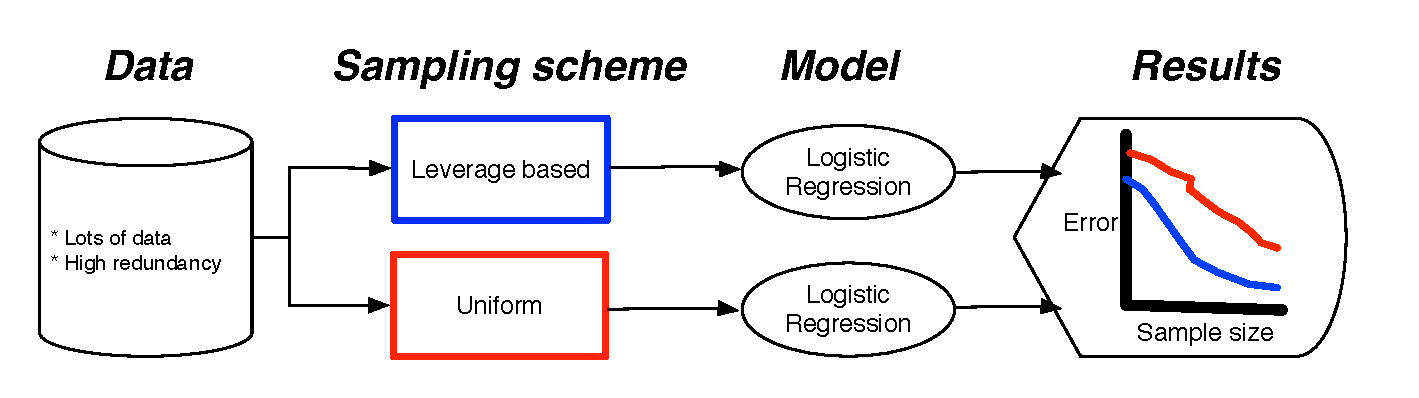
\includegraphics[width=.95\linewidth]{./02460_poster_template/images/ThoughtModel.eps}
\end{center}
%
\section{Research Questions}
\begin{itemize}
	\item Can we validate the results for least-squares regression shown by Ma et al. ?
	\item Will a linear regression based sampling distribution improve our performance in classification?
	\item Can leverage based sampling be generalized and used for classification?
\end{itemize}
%
\section{Datasets}
These datasets are drawn from distributions defined in Ma et al. \cite{Ma} and characterised by
\medskip
\begin{itemize}
	\item GA: Nearly uniform leverage-scores
	\item T3: Mildly non-uniform leverage-scores
	\item T1: Very non-uniform leverage-scores
\end{itemize}  
\medskip
\begin{figure}[H]
\centering
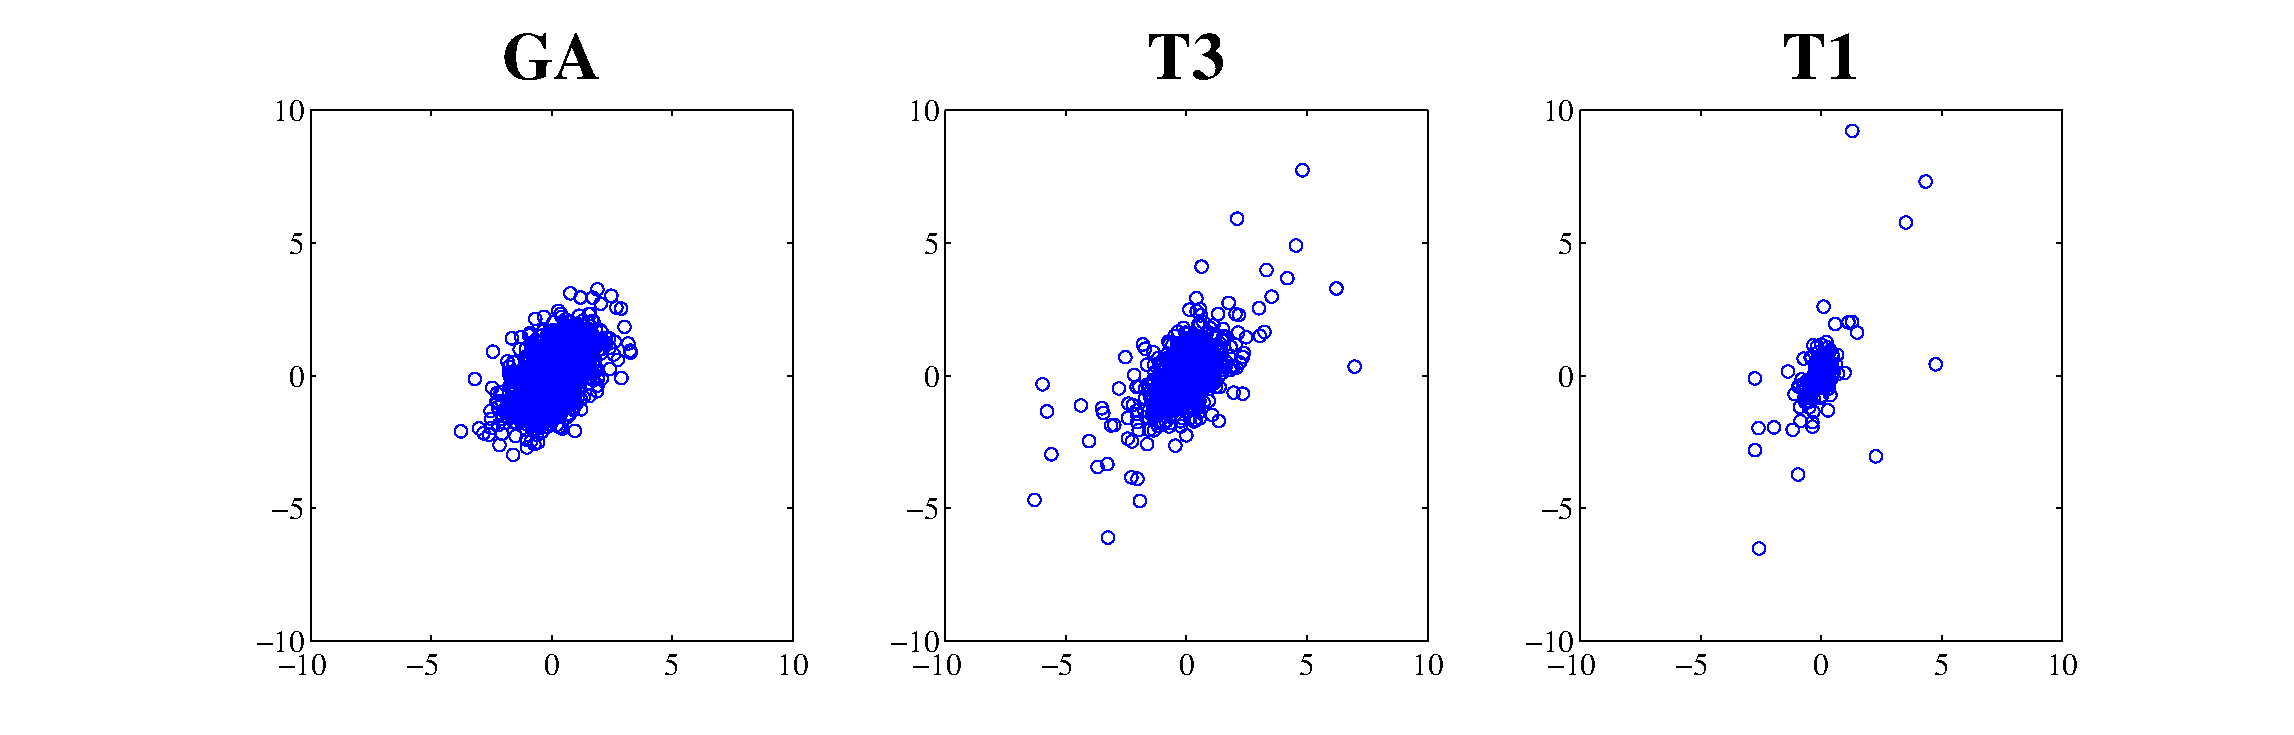
\includegraphics[width=\linewidth]{02460_poster_template/images/Data_distributions}
\caption{The three distributions considered standardized for comparison}
\end{figure}
%

\section{Leveraging for least-squares regression}
When fitting a model, we know that some datapoints are more important that others, leveraging is based on the idea that we can determine the importance of these point beforehand.
\medskip
\begin{enumerate}
\item A leverage-score is calculated for each datapoint (its importance).
\item These scores are normalized into a distribution $\pi$ to sample from.
\end{enumerate}
\medskip
Ma. et al. \cite{Ma} use the leverage-scores for least-square regression defined as the diagonal elements of
\begin{equation}
\H = \X \left( \X^T \X \right)^{-1} \X^T
 \label{eq:hdist}
\end{equation}
This comes from the closed form expression for predictions which is linear in $y$
\begin{equation*}
	\hat{\y}_n = \X_n*\hat{\beta} \quad \text{where} \quad \hat{\beta} = \left( \X^T \X \right)^{-1} \X^T \y 
\end{equation*}
\vspace{-1.3cm}
\section{Validation of the results  Ma et al.}
We have empirically tested and validated the results shown by Ma et al. \cite{Ma}.
\begin{figure}[H]
\centering
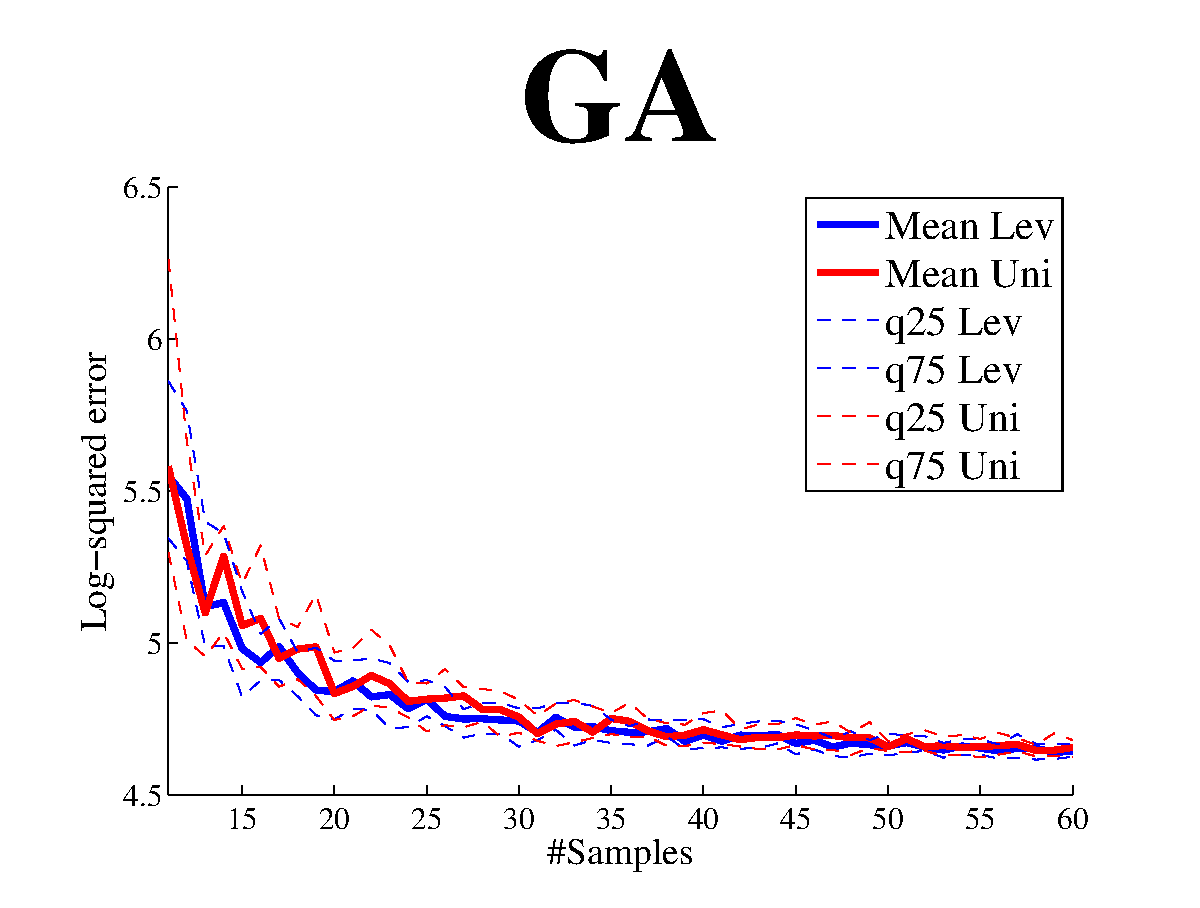
\includegraphics[width=.32\linewidth]{02460_poster_template/images/GALS.eps}
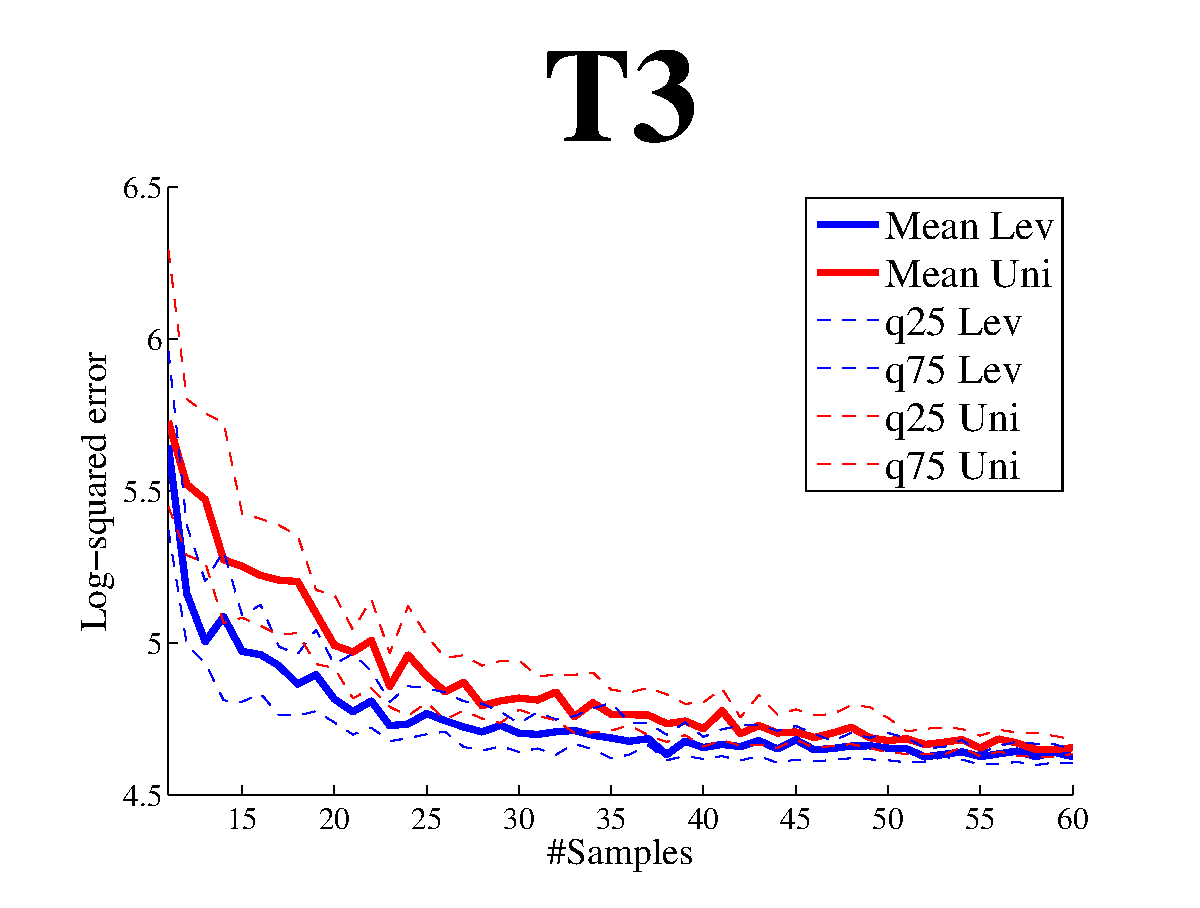
\includegraphics[width=.32\linewidth]{02460_poster_template/images/T3LS.eps}
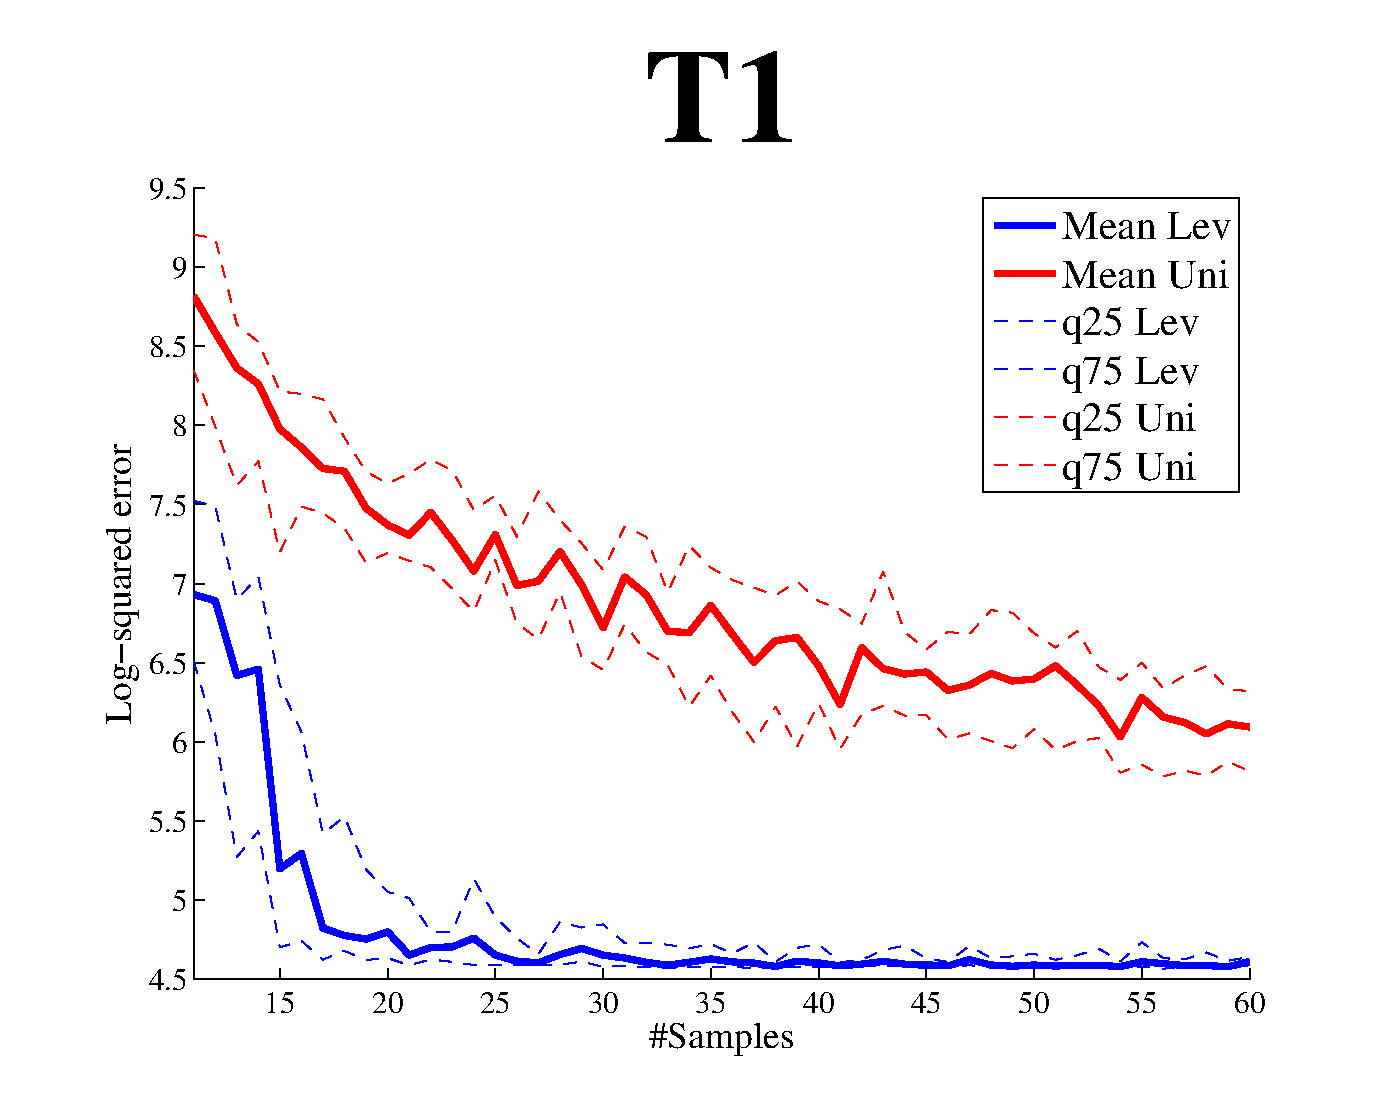
\includegraphics[width=.32\linewidth]{02460_poster_template/images/T1LS.eps}
\caption{Comparison of uniform {\bf\color{red}(red)} vs. leverage {\bf\color{blue}(blue)} based sampling schemes for least-squares regression. $N = 1000$, $d = 10$.}
\end{figure}
\begin{minipage}{.55\linewidth}
\begin{itemize}
\item GA: The leverage score are approximately uniform, and thus there is no significant difference between the two sampling schemes.
\item T3: Leveraging consistently provides slightly better results compared to uniform sampling.
\item T1: With \emph{very non-uniform} leverage-scores, leveraging clearly outperforms uniform sampling.
\end{itemize}
\end{minipage}
\hspace{.06\linewidth}
\begin{minipage}{.35\linewidth}
\begin{figure}[H]
    \caption{Comparison of sampling methods}
    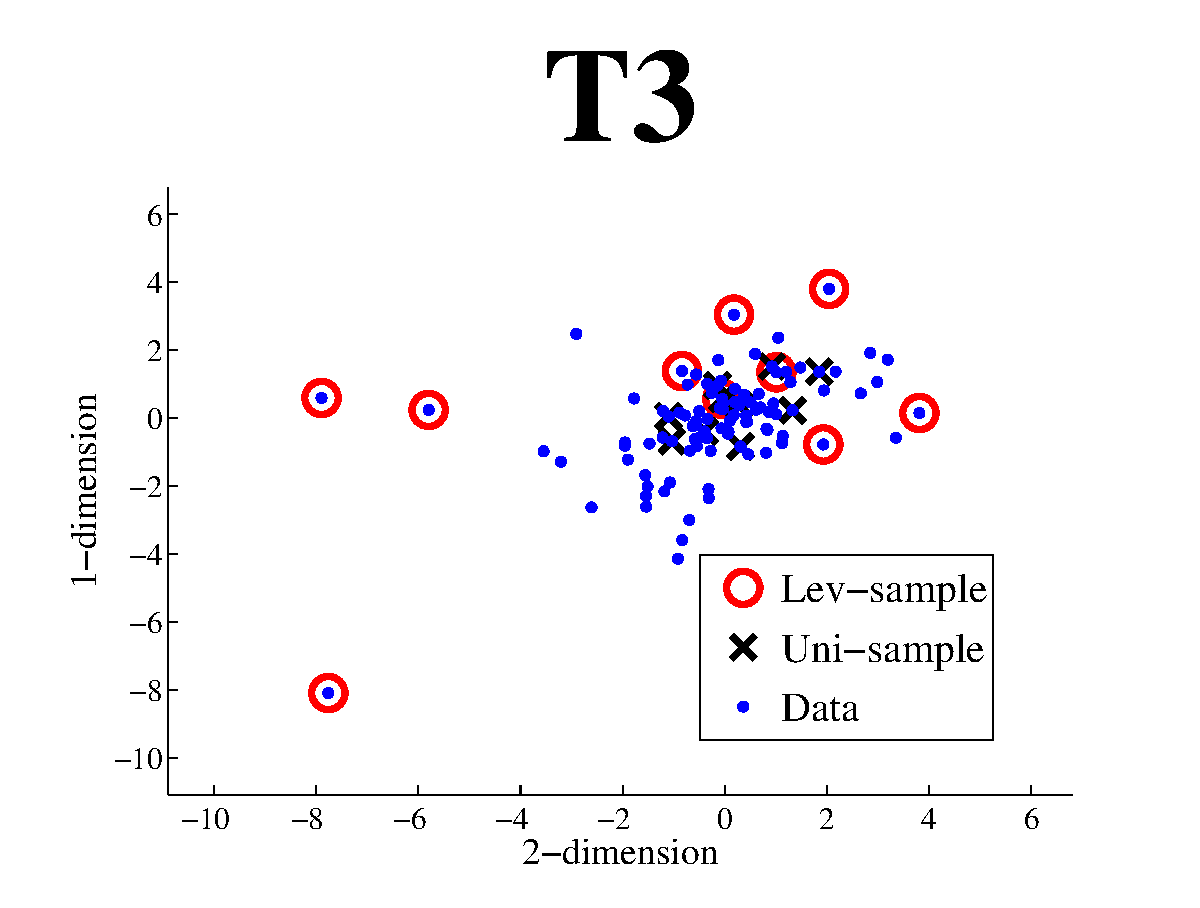
\includegraphics[width=.9\linewidth]{02460_poster_template/images/selection.eps}

\end{figure}
\end{minipage}

There results are consistent when varying $N$ and $d$, although the level of improvement varies.
%
\section{LS-based Distribution for Classification}

We sample from the same distribution \eqref{eq:hdist} as for least-squares regression. We use these samples to train a logistic regression model for 2 class classification, with equal class size.
  
\section{Test Results}
We compared the LS-distribution {\bf\color{blue}(blue)} to a uniform-distribution {\bf\color{red}(red)} in sampling for a logistic regression. The mean, 25th and 75th quantile are plotted.
\begin{figure}[H]
\centering
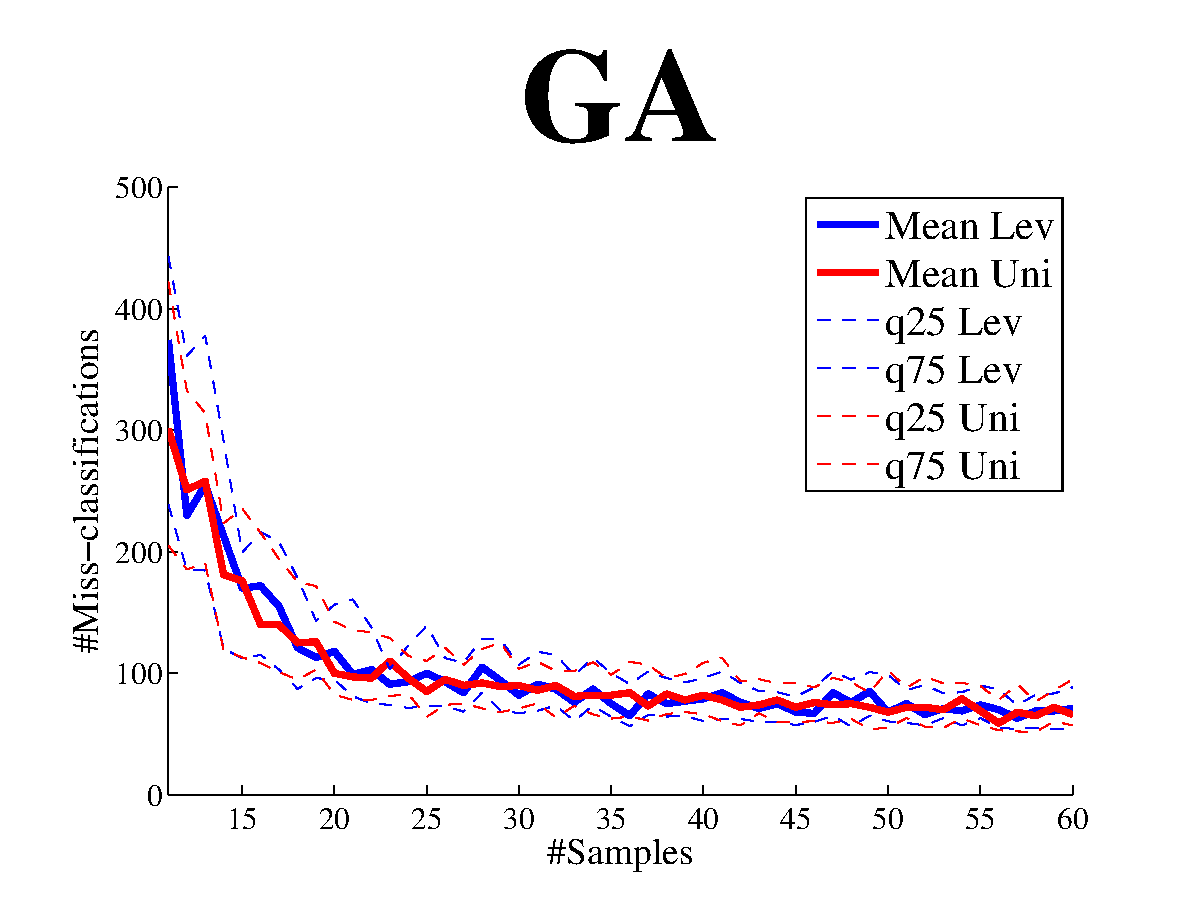
\includegraphics[width=.32\linewidth]{02460_poster_template/images/GA.eps}
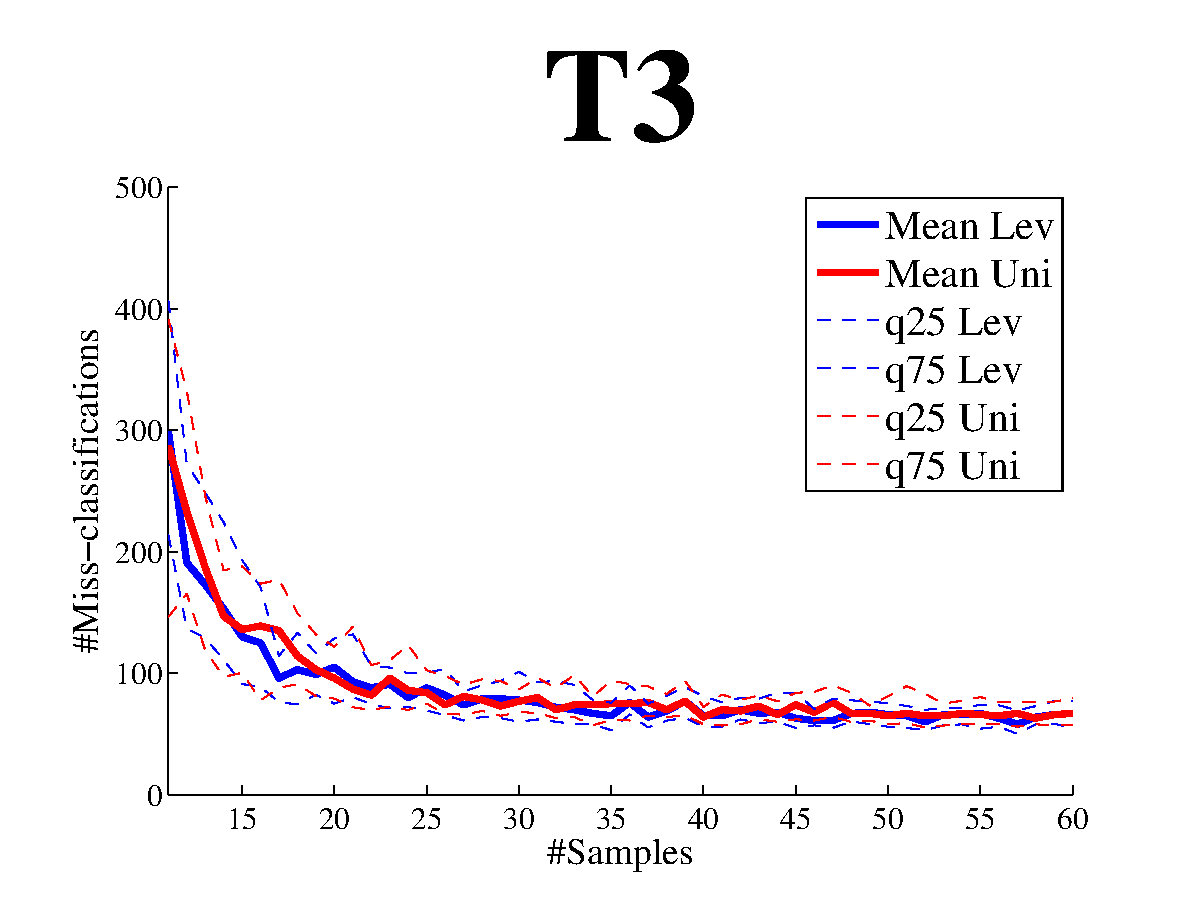
\includegraphics[width=.32\linewidth]{02460_poster_template/images/T3.eps}
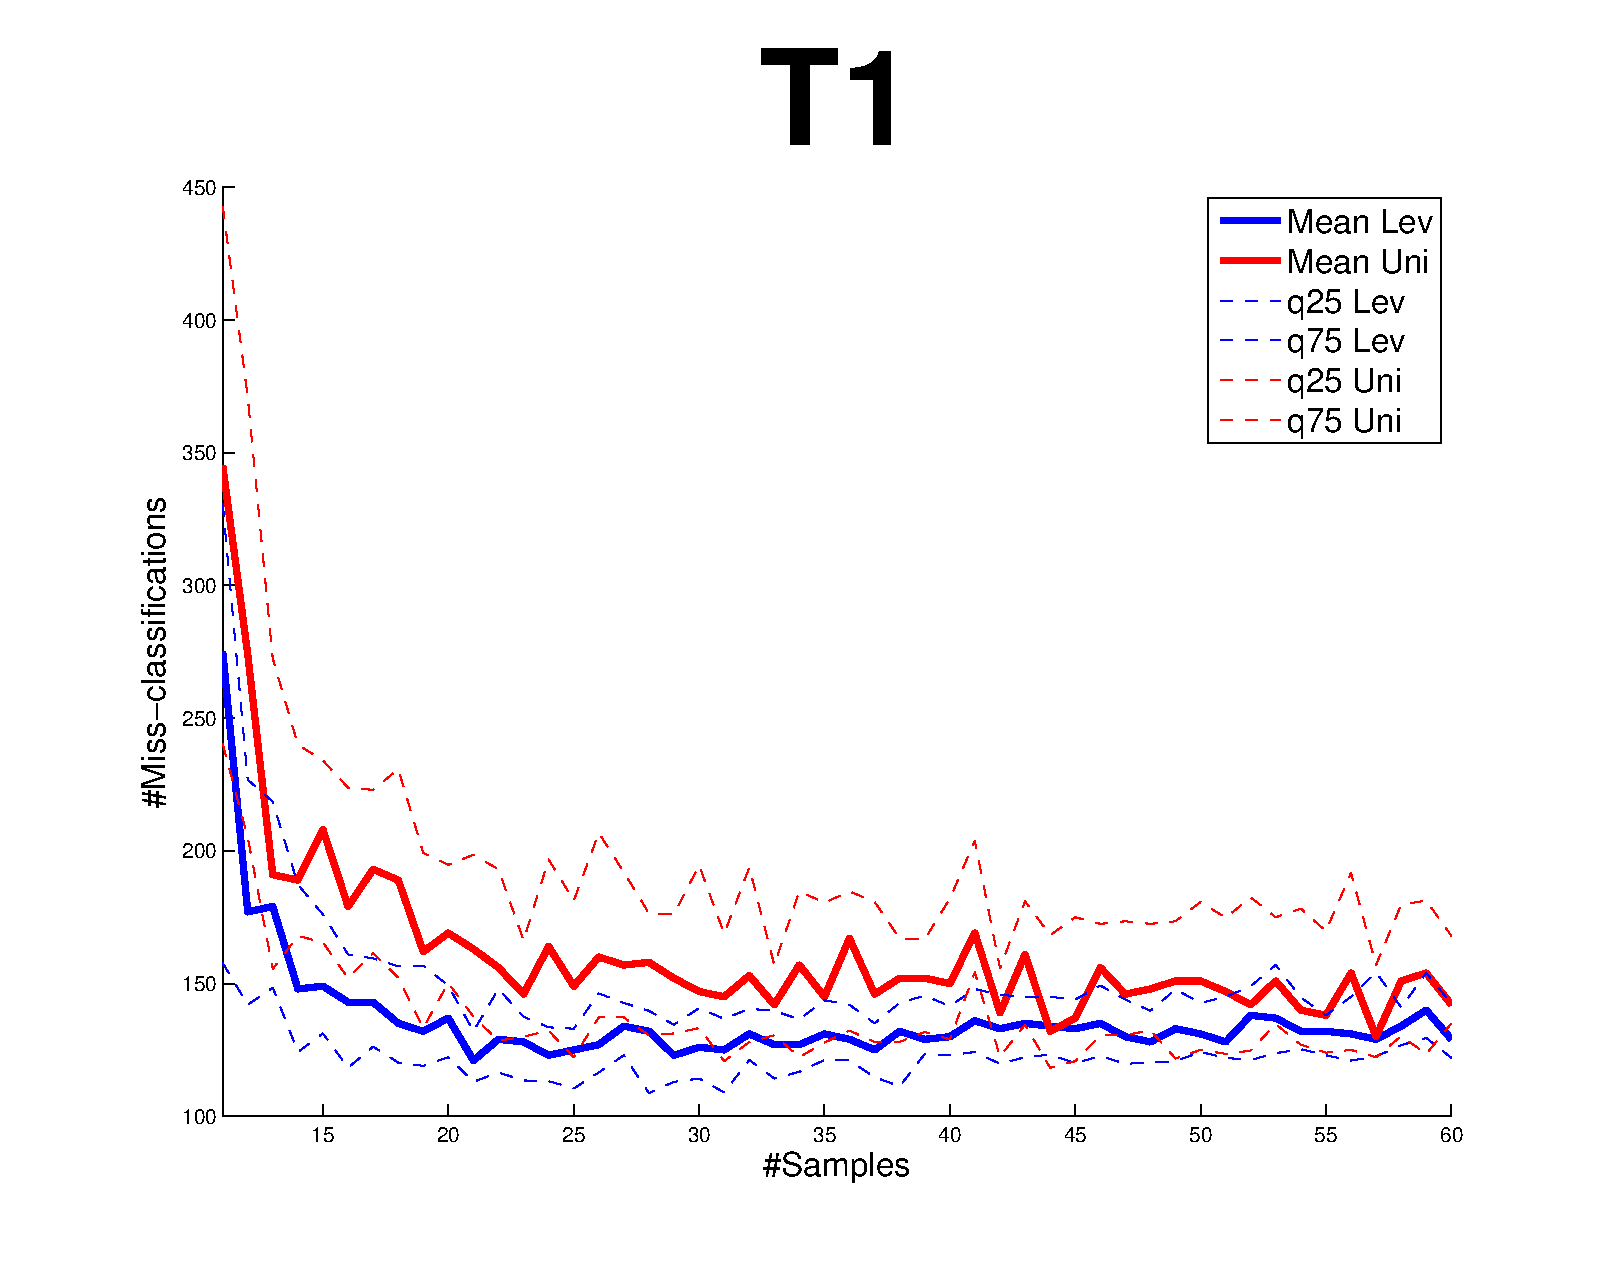
\includegraphics[width=.32\linewidth]{02460_poster_template/images/T1.eps}
\end{figure}	
\begin{itemize}
\item Sampling from the LS-distribution is no better that uniform on datasets of type GA and T3.
\item With very non-uniform leverage scores, T1, the LS-distribution slightly outperforms uniform sampling.
\end{itemize}
%It shows that a LS-distribution sample scheme, does not outperform a uniform-distribution for classification. 
The results shown are for dimension $p = 10$ and $N = 1000$ datapoints, but it is consistent when varying $p$ and $N$. \\
%

\section{Sensitivity Based Distribution}

We generalize the leverage scores to other models by seeing that they can be described as: 
	    \begin{equation}
	    \label{dyhatdy}
	    \frac{\delta \hat{\y}_n}{\delta \y_n} = Diag\left(H\right)
	    \end{equation}

Which we call the sensitivity of the model to a specific datapoint. For a general probabilistic discriminative model this requires the following:
    	\begin{equation}
    	 \hat{\y}_n = p(y|\bar{\x_n},\bar{\w}) \quad \bar{\w} \  \text{s.t.} \ \frac{\delta L}{\delta\bar{\w}}=0     	\label{optimum}
    	\end{equation}
Since \ref{optimum} depends both directly and indirectly on $y$ we see that
    	\begin{equation}
    	\frac{\delta}{\delta \y} \frac{\delta \mathcal{L}}{\delta \w} = 0 
    	\Rightarrow
    	\frac{\delta^2 \mathcal{L}}{\delta \y \delta \bar{\w}} + \frac{\delta^2 \mathcal{L}}{\delta \bar{\w} \delta \bar{\w}^T} \frac{\delta \bar{\w}}{\delta \y}= 0
    	\end{equation}
    	
    	and from this we can get our leverage-score \eqref{dyhatdy}
    	
    	\begin{equation*}
    		\frac{\delta \hat{\y}_n}{\delta \y_n}=\frac{\delta p(y|\bar{\x}_n,\bar{\w})}{\delta \bar{\w}^T} \frac{\delta \bar{\w}}{\delta \y} = - \frac{\delta p(y|\bar{\x}_n,\bar{\w})}{\delta \bar{\w}^T} \left[ \frac{\delta^2 \mathcal{L}}{\delta \bar{\w} \delta \bar{\w}^T} \right]^{-1} \frac{\delta^2 \mathcal{L}}{\delta \y \delta \bar{\w}}
    	\end{equation*}
    	
    	When using this model, initial weights are found by fitting a small uniform sample. This is expected outperform LS-based sampling since it introduces dependence on class information.
%
\section{Test results}
\vspace{-30pt}
\begin{figure}[H]
\centering
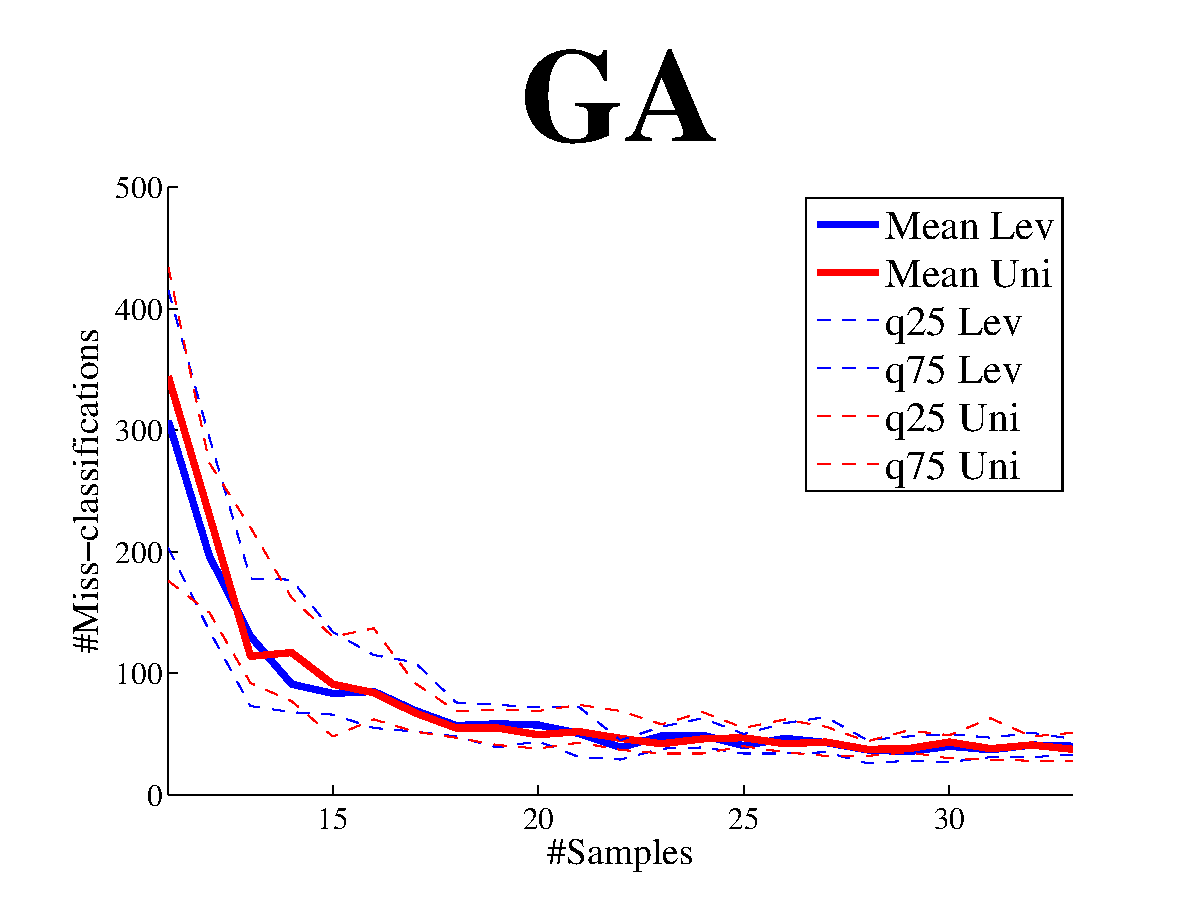
\includegraphics[width=.32\linewidth]{02460_poster_template/images/GAsen.eps}
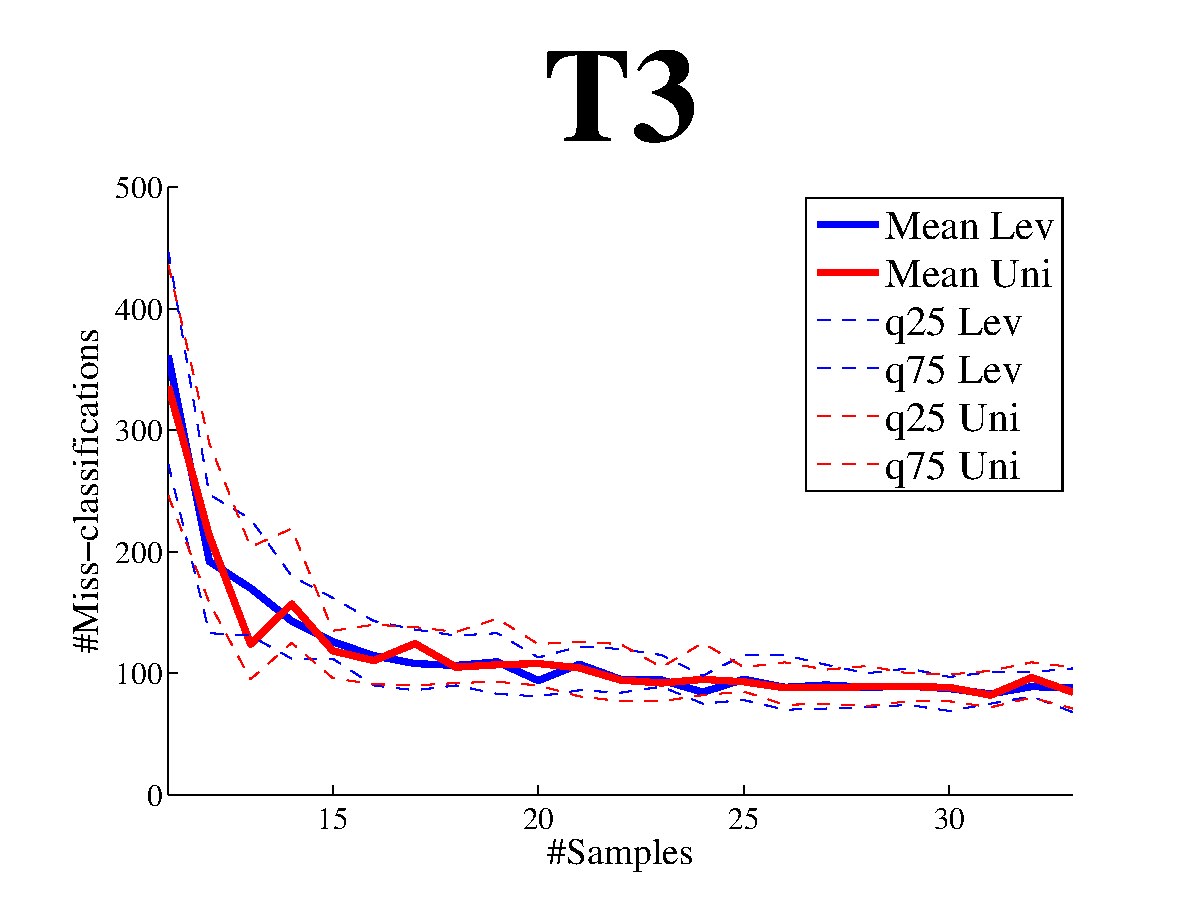
\includegraphics[width=.32\linewidth]{02460_poster_template/images/T3sen.eps}
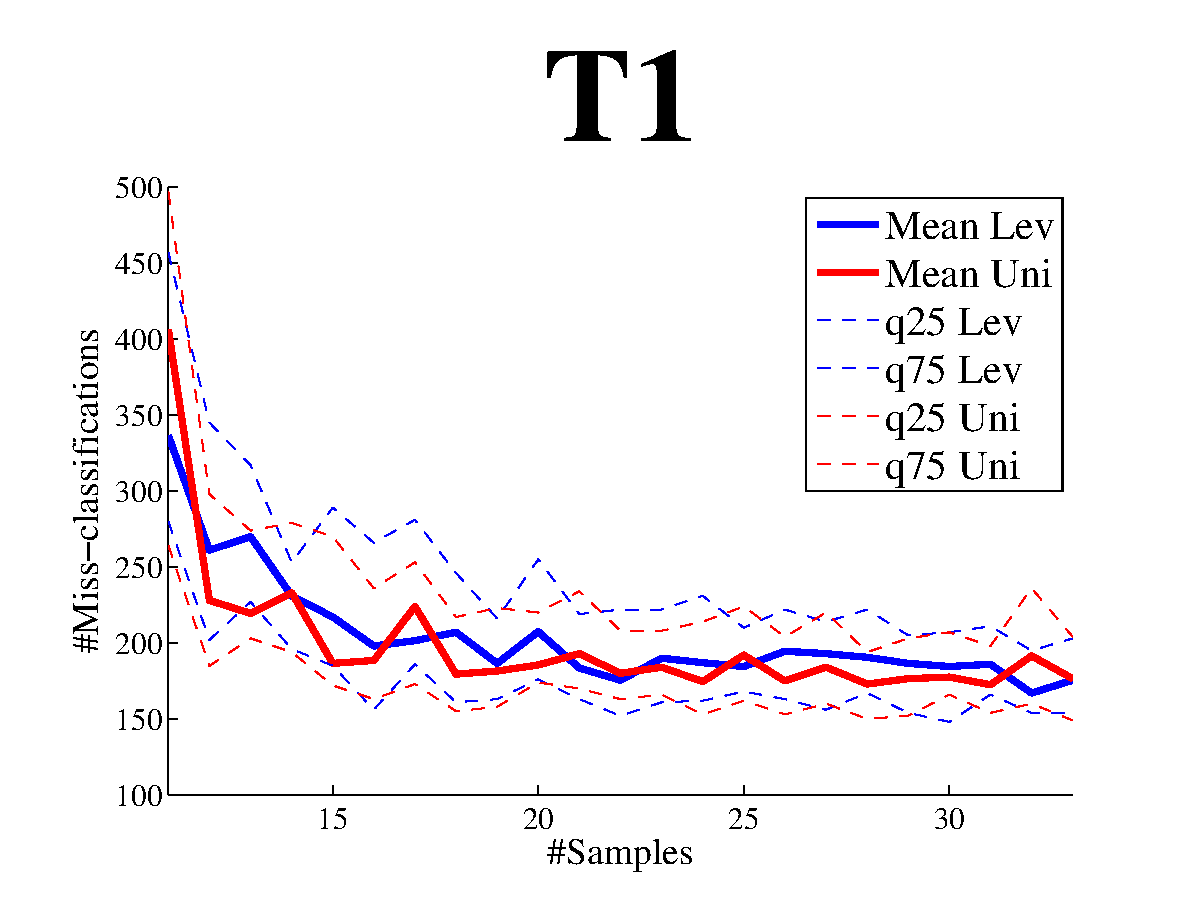
\includegraphics[width=.32\linewidth]{02460_poster_template/images/T1sen.eps}
\caption{Comparison of sensitivity vs. uniform -based sampling for logistic regression.}
\end{figure}	

We see that the \emph{sensitivity based sampling} gives us a performance  equivalently to that of uniform sampling.
%
\section{Future work}
From our work several new question arise.
\begin{itemize}
\item How large show the initial sampling size be for sensitivity-based sampling?
\item How should the non-linear sensitivity based leverage scores be normalised? 
\item Should all points be sampled from the initial weights found, or should the process be iterative?
\end{itemize}
%
\section{Conclusion}
In the case of linear regression, leverage-based sampling provides a improvement over uniform sampling when the leverage-scores are mildly or very non-uniform.

Using the LS-based sampling for classification is slightly better with very non-uniform leverage-scores, T1 data.
%Using the LS-based sampling for classification shows no improvement on datasets \emph{GA} and \emph{T3}, but for \emph{T1} with very non-uniform leverage-scores, the approach is slightly better.

We have generalized the concept of leverage-based scores to classification with logistic regression and it has shown no improvements. However further analysis and tweaking might improved this approach.
%The LS-based leverage sampling gives no advantage over uniform sampling and generally performs worse. LS-distribution is based on what is important for linear regression, it does not have an advantage in finding important points for classification.

\section{References}
%
\vspace{-2.5cm}
\bibliographystyle{is-unsrt}
%\footnotesize{
\bibliography{./mlbib}
%}

\appendix

\section{The derivative of prediction or Sensitivity}
We wish to find the effect that a datapoint's class has on the predicted class for that datapoint.
\begin{equation}
\label{dyhatdy}
\frac{\delta \hat{Y}_n}{\delta Y_n}
\end{equation}

Our prediction is 
\begin{equation}
 \hat{Y}_n = p(y|\bar{x},\bar{w})
\end{equation}
where $\bar{w}$ is subject to 
\begin{equation}
\label{optimum}
\frac{\delta L}{\delta\bar{w}}=0
\end{equation}
Which means that we have found a locally optimal solution.

We now assume that when we move $y$ by a small amount $\delta y$ then \ref{optimum} still holds.

Essentially assuming some smoothness around the optimum.

Using this and the fact that \ref{optimum} depends both directly and indirectly on y we see that

\begin{eqnarray*}
&\frac{\delta}{\delta y} \frac{\delta L}{\delta w} = 0\\
\Downarrow & \\
&\frac{\delta^2 L}{\delta y \delta \bar{w}} + \frac{\delta^2 L}{\delta \bar{w} \delta \bar{w}^T} \frac{\delta \bar{w}}{\delta y}= 0
\end{eqnarray*}

and from this we can isolate

\begin{equation}
\label{dwdy}
\frac{\delta \bar{w}}{\delta y} = - \left[ \frac{\delta^2 L}{\delta \bar{w} \delta \bar{w}^T} \right]^{-1} \frac{\delta^2 L}{\delta y \delta \bar{w}} 
\end{equation}

Rewriting \ref{dyhatdy} we get

\begin{equation}
\frac{\delta \hat{Y}_n}{\delta Y_n} = \frac{\delta p(y|\bar{x},\bar{w})}{\delta Y_n} =  \frac{\delta p(y|\bar{x},\bar{w})}{\delta \bar{w}^T} \frac{\delta \bar{w}}{\delta y}
\end{equation}

And inserting \ref{dwdy} 

\begin{equation}
\frac{\delta p(y|\bar{x},\bar{w})}{\delta \bar{w}^T} \frac{\delta \bar{w}}{\delta y} = - \frac{\delta p(y|\bar{x},\bar{w})}{\delta \bar{w}^T} \left[ \frac{\delta^2 L}{\delta \bar{w} \delta \bar{w}^T} \right]^{-1} \frac{\delta^2 L}{\delta y \delta \bar{w}}
\end{equation}


\section{Randomised algorithm}
\emph{Uncertainty based on asymptotic likelihood and $\bar{w}$-distribution}\\
Let $\mathcal{L}_\infty$ be the log-likelihood function for a distribution, now let $\mathcal{L}_N$ denote the log-likelihood function based on $N$ observations from this distribution. Furthermore, let $N$ be a large number, for which $L_N \approx L_\infty$. 

\begin{equation}
\mathcal{L_N} = \frac{1}{N} \sum_{n=1}^N \ell_n \qquad \bar{w} \, s.t. \, \frac{\delta \mathcal{L}}{\delta \bar{w}} = \bar{0} \label{eq:ra1}
\end{equation}
Where $\ell_n$ is the log-likelihood of the $n^{th}$ observation. And $\bar{w}$ is the true weights for the distribution, then we combine the expressions from \eqref{eq:ra1}, such that for the true weights the following must be fulfilled:

\begin{equation}
\frac{1}{N} \sum_{n = 1}^N \frac{\delta \ell_n}{\delta \bar{w}} = 0 \label{eq:ra2}
\end{equation}

\emph{(Skal vi lige skrive lidt om at $\Delta w = w-w_0$ og er en lille forskydelse i vægtene? Eller er det en lille forskydelse?) }
For each of the $N$ observations, we can approximate the log-likelihood of the $n^{th}$ observation with this taylor expansion:

\begin{equation}
\ell_n(\bar{w}) = 
\ell_n\left(\bar{w}_0 \right) + 
\left. \frac{\delta \ell_n}{\delta \bar{w}} \right|_{\bar{w}_0} \Delta \bar{w} + 
\frac{1}{2} Tr \left[ \left. \frac{\delta \ell_n}{\delta \bar{w} \delta \bar{w}^T} \right|_{\bar{w}_0} \Delta \bar{w} \Delta \bar{w}^T \right] \label{eq:loglihood-oneObs}
\end{equation}
Or for the entire log-likelihood function: \textbf{Where did the trace go ?}
\begin{equation}
\mathcal{L}_N(\bar{w}) = 
\mathcal{L}_N\left(\bar{w}_0\right) + 
\left(\left.\frac{\delta \mathcal{L}_N}{\delta \bar{w}}\right|_{\bar{w}_0} \right)^T \cdot \Delta \bar{w} +
\frac{1}{2} \Delta \bar{w}^T \left( \left. \frac{\delta^2 \mathcal{L}_N}{\delta \bar{w} \delta \bar{w}^T}\right|_{\bar{w}_0} \right) \Delta \bar{w} + R \label{eq:entireLogLike}
\end{equation}
Where $R$ is the error of the approximation and assumed to be 0. Furthermore, we define $\bar{\bar{H}}_N = \left. \frac{\delta^2 \mathcal{L}_N}{\delta \bar{w} \delta \bar{w}^T}\right|_{\bar{w}_0}$, and $\bar{g}:N = \left.\frac{\delta \mathcal{L}_N}{\delta \bar{w}}\right|_{\bar{w}_0}$. And evaluate condition \eqref{eq:ra1} on $\bar{w}$:
\begin{equation}
\frac{\delta \mathcal{L_N}}{\delta \bar{w}} = \bar{g}_N+\bar{\bar{H}}_N \Delta \bar{w} = \bar{0}
\end{equation}
We replace $\Delta \bar{w}$ with $\hat{\Delta \bar{w}}$  as $N$ is a finite number, thus only approximating $\Delta \bar{w}$. Isolating $\hat{\Delta \bar{w}}$, and using Ljung \textbf{[REFERENCE?]}, we get: \textbf{Is this to soon to involve Ljung?}
\begin{equation}
\hat{\Delta \bar{w}} = - \bar{\bar{H}}_N^{-1} \cdot \bar{g}_N \overbrace{=}^{Ljung} -\bar{\bar{H}}
_0^{-1} \cdot \bar{g}_{\bar{w}} \left( \bar{w}_0 \right)
\end{equation}
\emph{(Forklaring af at $H_0$ er uafhængig af datasæt, mens $g$ nu er afhængig af $w$ evalueret i $w_0$)}
Besides getting an estimate for $\hat{\Delta \bar{w}}$, we can find the mean of the distribution:
\[
\left\langle \hat{\Delta \bar{w}} \right\rangle = - \bar{\bar{H}}_0^{-1} \bar{g}_0 = 0
\]
As $\delta \bar{w} = \bar{w}-\bar{w}_0$ ??mistet tråden?

\subsection{Covariance of $\bar{w}$ - distribution}


\textbf{Why do we do this???}

\begin{equation}
\left\langle \delta \bar{w} \delta \bar{w}^T \right\rangle_{N} = 
\left\langle \bar{\bar{H}}^{-1} \bar{g} \bar{g}^T \bar{\bar{H}}^{-1} \right\rangle
\overbrace{=}^{Ljung} \bar{\bar{H}}^{-1}_0 \left\langle \bar{g}\bar{g}^T \right\rangle \bar{\bar{H}}^{-1}_0 + R'
\end{equation}
With error $R' = O\left(\frac{1}{N}\right) \approx 0$, for large $N$. We look at the covariance of the gradient function
\begin{align}
\left\langle \bar{g} \bar{g}^T \right\rangle_N &= 
\frac{1}{N^2}\sum_{n, n' = 1}^N \left\langle \left. \frac{\delta \ell_n}{\delta_n \bar{w}} \right|_{\bar{w}_0} \left.\frac{\delta \ell_{n'}}{\delta_n \bar{w}} \right|_{\bar{w}_0} \right\rangle\\
 & = \frac{1}{N^2} \left(\sum_{n \neq n'} \underbrace{\left\langle \left. \frac{\delta \ell_n}{\delta \bar{w}} \right|_{\bar{w}_0} \right\rangle \cdot \left\langle \left. \frac{\delta \ell_{n'}}{\delta \bar{w}^T} \right|_{\bar{w}_0} \right\rangle }_0
 + \sum_{n =1 }^N \left\langle \left. \frac{\delta \ell_n}{\delta \bar{w}} \right|_{\bar{w}_0} \left. \frac{\delta \ell_n}{\delta \bar{w}^T} \right|_{\bar{w}_0}  \right\rangle \right)
\end{align}
Due to the assumption of independence, only the $N$ diagonal elements are non-zero. So;
\begin{equation}
\left\langle \bar{g} \bar{g}^T \right\rangle_N = \frac{1}{N} \left\langle \left. \frac{\delta \mathcal{L}}{\delta \bar{w}} \right|_{\bar{w}_0} \left. \frac{\delta \mathcal{L}}{\delta \bar{w}^T} \right|_{\bar{w}_0}  \right\rangle \label{eq:gg}
\end{equation}


\subsection{Proof that $\left\langle \left. \frac{\delta \mathcal{L}}{\delta \bar{w}} \right|_{\bar{w}_0} \left. \frac{\delta \mathcal{L}}{\delta \bar{w}^T} \right|_{\bar{w}_0}  \right\rangle = \bar{\bar{H}}_0$ }
Tekst test
\begin{equation}
\left\langle \bar{g} \bar{g}^T \right\rangle_N = 
\frac{1}{N^2} \sum_{n = 1}^N \int_{\Omega} 
\left. \frac{\delta \ell_n({\bar{x})}}{\delta \bar{w}} \right|_{\bar{w}_0}
\left. \frac{\delta \ell_n({\bar{x})}}{\delta \bar{w}} \right|_{\bar{w}_0}
p(\bar{x}) \delta x \label{eq:ggx}
\end{equation}
From \eqref{eq:gg} and \eqref{eq:ggx}, and setting $ \ell_n({\bar{x})} = p(\bar{x})$:
\begin{align}
\left.\bar{\bar{H}} \right|_{\bar{w}_0} &= 
\frac{1}{N} \sum_{n = 1}^N \int_{\Omega} 
\frac{\delta}{\delta \bar{w} \delta \bar{w}^T}
- \log p\left(\bar{x} \middle| \bar{w} \right) p(\bar{x}) \delta x\\
 &= \frac{1}{N} \sum_{n = 1}^N \int_{\Omega} - \frac{\delta}{\delta \bar{w}} \frac{1}{p\left(\bar{x}\right)}\frac{\delta }{\delta \bar{w}^T} p(\bar{x} | \bar{w}) p(\bar{x}) \delta \bar{x}\\
\end{align}
Now if $p(\bar{x}|\bar{w}_0) = p(x)$, then

\subsection{Uncertainty of prediction}
For a number of weight-vectors $\bar{w}$, we take the mean of predictions based on these weight-vectors;
\begin{equation}
\left\langle p \left(y \middle| \bar{x}, \bar{w} \right) \right\rangle \approx p \left(y \middle| \bar{x}, \hat{\bar{w}} \right) = p \left(y \middle| \bar{x}, \mathbf{E}(\bar{w}) \right)
\end{equation}
We now look at a small change in the prediction $\Delta p$, caused by a change of $\Delta \bar{w}$ in true weight vector $\bar{w}_0$. 
\begin{equation}
\Delta p = p \left(y \middle| \bar{x}, \bar{w}_0+\Delta \bar{w} \right)
- p \left(y \middle| \bar{x}, \bar{w}_0 \right) 
\approx \left.\frac{\delta p}{\delta \bar{w}} \right|_{w_0}\cdot \Delta \bar{w}
\end{equation}
The variance of $\Delta p$, can then be computed as
\begin{equation}
\left\langle (\Delta p)^2 \right\rangle = Tr\left[ 
\frac{\delta p}{\delta \bar{w}} \left(\frac{\delta p}{\delta \bar{w}}\right)^T
\left\langle \Delta \bar{w} \Delta \bar{W}^T \right\rangle \right]
= \frac{1}{N} \left(\frac{\delta p}{\delta \bar{w}}\right)^T 
 \bar{\bar{H}}^{-1} \frac{\delta p}{\delta \bar{w}}
\end{equation}

\subsubsection{For a linear model with known $\sigma^2$}
The prediction in a linear model is:
\begin{equation}
p(y|\bar{x},\bar{w}) = \frac{1}{\sqrt{2 \pi \sigma^2}} e^{\frac{(y-f(\bar{x|}|\bar{w})}{2 \sigma^2}} \label{linearprediction}
\end{equation}
Where $y$ is the target and $f(\bar{x|}|\bar{w})$ is the prediction. Differentiating \eqref{eq:linearprediction} with respect to $\bar{w}$: \emph{(Hvorfor er det vi gør det??)}
\begin{equation}
\frac{\delta p}{\delta w} = \frac{1}{\sqrt{2 \pi \sigma^2}} e^{-\frac{(y-f(\bar{x}|\bar{w})^2}{2\sigma^2}}-(y-f(\bar{x}|\bar{w}) \frac{\delta f(\bar{x}|\bar{w})}{\delta \bar{w}}
\end{equation}
We let $y = f(\bar{x}|\bar{w})+ \epsilon$. (Targets kan beskrives som en approximativ funktion + en fejl ..)
\begin{equation}
\frac{\delta p}{\delta \bar{w}} = \underbrace{ 
\frac{1}{\sqrt{2\pi \sigma^2}}
e^{-\frac{\epsilon^2}{2 \sigma^2}}\epsilon^2
}_{\texttt{const. w.r.t. } \bar{x} 
} 
\frac{\delta f(\bar{x}|\bar{w})}{\delta \bar{w}}^T \bar{\bar{H}}_0^{-1} \frac{\delta f(\bar{x}|\bar{w})}{\delta \bar{w}}
\end{equation}

\newpage
\section{Logbook}

\subsection*{Learning objectives}

\subsection*{Overall Project Goals/Delimitation/Hypotheses}

\subsection*{General stuff}



\subsection*{Week 1 (9): 24.02.2014 - 02.03.2014}
\subsubsection*{Project meeting}
No project meeting was possible this week, and we had yet to decided between 
\begin{enumerate}
\item Randomized algorithms: \\
\emph{A Statistical Perspective on Algorithmic Leveraging, Ping Ma, Micheal W. Mahoney, Bin Yu}.  $http://arxiv.org/abs/1306.5362$
\item Spectral learning of HMMs:\\
\emph{A Method of Moments for Mixture Models and Hidden Markov Models}. A. Anandkumar, D. Hsu, and S.M. Kakade. Preprint, Feb. 2012 : $http://newport.eecs.uci.edu/anandkumar/pubs/AnandkumarEtal_mixtures12.pdf$
\end{enumerate}

We spend the week getting an overview of the articles and the projects.

\subsection*{Week 2 (10): 03.03.2014 - 09.03.2014}
\subsubsection*{Project meeting}
\textbf{Questions:}\\
\begin{itemize}
\item What is the idea behind leveraging for least-squares regression?
\item Can we generalise the idea to general?
\item Can leveraging improve performance in video screen classification?
\item Video classification e.g. faces, emotions, gender.
\end{itemize}

\textbf{Implementation:}\\
No implementation at this point.

\textbf{Results:}\\
No results at this time.

\textbf{Decisions:}\\
Gain a better understanding of the underlying idea of leveraging, by watching a talk on \emph{Statistical Leverage and Improved Matrix Algorithms} by M. W. Mahoney ($http://videolectures.net/icml09_mahoney_itslima/$). And analyses the results for 

\subsubsection*{Updated Project Goals and Delimitation}
\begin{itemize}
\item Validation of the results shown by Ma. et al.
\item Can we generalise the idea of leveraging for a general likelihood funktion?
\end{itemize}

\subsection*{Week 3 (11): 10.03.2014 - 16.03.2014}
\subsubsection*{Project meeting}
\textbf{Questions:}\\
\begin{itemize}
\item How does the leverage scores look for LS-regression? (Plotting $H_{n,n}$ vs. $||x_n||$)
\end{itemize}
\textbf{Implementation:}\\
No implementation at this point.

\textbf{Results:}\\
\begin{itemize}
\item The general idea of leveraging is to identify how the estimated value $\hat{\y}$ relates to the targeted value $\y$. Which for LS-regression is $\hat{\y} = H \y$.
\end{itemize}

\textbf{Decisions:}\\

\subsubsection*{Updated Project Goals and Delimitation}
\begin{itemize}
\item Can we generalise the expression $\hat{\y} = H \y$ to logistic regression?
\end{itemize}

\subsection*{Week 4 (12): 17.03.2014 - 23.03.2014}
\subsubsection*{Project meeting}
\textbf{Questions:}\\
\begin{itemize}
\item How are the distributions used by Ma. et al. calculated?
\item Finding emotional faces datasets.
\end{itemize}

\textbf{Implementation:}\\
\begin{itemize}
\item Finding leverage-scores for LS-regression
\item Solving LS-regression when comparing uniform- to leverage-based sampling.
\item Illustrating leverage scores ($H_{n,n}$ vs. $||x_n||$)
\end{itemize}

\textbf{Results:}\\
Initial results promising, but only single run performance between uniform- and leverage-based sampling.

\textbf{Decisions:}\\

\subsubsection*{Updated Project Goals and Delimitation}
\begin{itemize}
\item We want to validate the results of Ma et. al. empirically.
\item In video classification we want to do binary classification of \emph{happy} and \emph{sad} faces.
\end{itemize}


\subsection*{Week 5 (13): 24.03.2014 - 30.03.2014}
\subsubsection*{Project meeting}
\textbf{Questions:}\\
\begin{itemize}
\item Will using the leverage-scores for LS-regression improve our performance in binary classification?
\end{itemize}

\textbf{Implementation:}\\
\begin{itemize}
\item The three distributions $GA$,$T3$ and $T1$ are implemented, and tested for linear regression.
\item Learning curves and test-framework for LS-regression, used for testing the results show by Ma et al.
\end{itemize}

\textbf{Results:}\\
\begin{itemize}
\item We get comparable results on LS-regression to those shown by Ma et al.
\item A leverage-based sampling does not improve for GA-type data, as the leverage scores are approximately uniform, thus there are no "important" datapoints that can be sampled.
\item A leverage-based sampling for T3-type data consistently performs better or equal to a uniform sampling. Although the performance increase modest.
\item A leverage-based sampling for T1-type data also consistently outperforms a uniform-based sampling, this is expected as the T1 data have very non-uniform leverage scores i.e. "important" datapoints. 
\end{itemize}

\textbf{Decisions:}\\
Generalisation of the leverage-based sampling scheme $\frac{\delta \hat{\y}}{\delta \y}$ to logistic regression, as well as a sampling distribution based on the uncertainty of the predictions (asymptotic theory) is to be done by Lars Kai.

\subsubsection*{Updated Project Goals and Delimitation}
\begin{itemize}
\item Will using the leverage-scores for LS-regression improve our performance in binary classification?
\item We have validated the results of Ma et al. for LS-regression on $GA$,$T3$ and $T1$ distributed data.
\end{itemize}
\subsection*{Week 6 (14): 31.03.2014 - 06.04.2014}
\subsubsection*{Project meeting}
%\textbf{Questions:}\\

\textbf{Implementation:}\\
\begin{itemize}
\item Three distributions for binary classification data, also named $GA$, $T3$ and $T1$ which represent respectively classification data with nearly uniform, moderately non-uniform and very non-uniform leverage-scores.
\item Learning curves for logistic regression based on uniform or LS-regression leverage-scores.
\end{itemize}

\textbf{Results:}\\
Initial results using leverage-scores based on LS-regression shows no improvement on GA-type (expected) and performs significantly worse on T3- and T1-type data.

Lars Kai has derived a generalised expression $\frac{\delta \hat{\y}}{\delta \y}$ for a general likelihood function. As well as the uncertainty based sampling approach.

\textbf{Decisions:}\\
Lars Kai gathers his scribles on the back of some insignificant article in a form that is easier to read and follow.

Our full focus is now on midterm preparation.

\subsubsection*{Updated Project Goals and Delimitation}
\begin{itemize}
\item Compare uniform sampling to a leverage based distribution (generalisation) and a uncertainty based distribution.
\end{itemize}

\subsection*{Week 7 (15): 07.04.2014 - 13.04.2014}
\subsubsection*{Project meeting}
Discussion about the midterm and improvements that should be done.

%\textbf{Questions:}\\

%\textbf{Implementation:}\\

%\textbf{Results:}\\

%\textbf{Decisions:}\\

%\subsubsection*{Updated Project Goals and Delimitation}



\subsection*{Week 8 (16): 14.04.2014 - 20.04.2014}
Easter, no project meeting, but sporadic work was done, mostly clarification and bug-finding.


\subsection*{Week 9 (17): 21.04.2014 - 27.04.2014}\subsubsection*{Project meeting}
%\textbf{Questions:}\\

%\textbf{Implementation:}\\

\textbf{Results:}\\
Lars Kai gives us a copy and explains the general concepts behind the generalisation of $\frac{\delta \hat{\y}}{\y}$ and uncertainty-based sampling.

\textbf{Decisions:}\\
We are to understand and digitalise the results derived.

%\subsubsection*{Updated Project Goals and Delimitation}



\subsection*{Week 10 (18): 28.04.2014 - 04.05.2014}
\subsubsection*{Project meeting}
\textbf{Questions:}\\

%\textbf{Implementation:}\\

\textbf{Results:}\\

\textbf{Decisions:}\\

%\subsubsection*{Updated Project Goals and Delimitation}



\subsection*{Week 11 (19): 05.05.2014 - 11.05.2014}
\subsubsection*{Project meeting}
\textbf{Questions:}\\

\textbf{Implementation:}\\

\textbf{Results:}\\

\textbf{Decisions:}\\

\subsubsection*{Updated Project Goals and Delimitation}



\subsection*{Week 12 (20): 12.05.2014 - 18.05.2014}
\subsection*{Week 13 (21): 19.05.2014 - 25.05.2014}
\subsection*{Week 14 (22): 26.05.2014 - 01.06.2014}







\end{document}